\chapter{Biological inspiration}

\section{McCulloch-Pitss neuron}
The model aims to represent a basic neuron, that receives a signal from the $N$ neighbouring neurons (as we can see in Figure \ref{fig:MPneuron}), whose state is represented by the vector $x=(x_1, x_2, \ldots, x_N)$ and which are associated to a synaptic weight vector $J=(J_1, J_2, \ldots, J_N)$; the neuron elaborates this information an returns as output the variable $y$
\begin{equation}\label{eq:MPneuron}
    y= \theta\left(\sum\limits_{j=1}^N J_j x_j - U^* \right)  
\end{equation}
where $\theta$ is the Heavyside function and $U^*$ is the \tbf{activation threshold of the neuron}.

\begin{definicion}(Heavyside function)
    The main purpose of the \tbf{Heavyside function} is to switch something on or off depending on whether the input is positive or not. Formally, it is defined as
    \begin{equation*}
        \theta(x) = \begin{cases}
            1 & \text{if } x \geq 0 \\
            0 & \text{if } x < 0
        \end{cases}
    \end{equation*}
\end{definicion}

\begin{figure}[H]
    \centering
    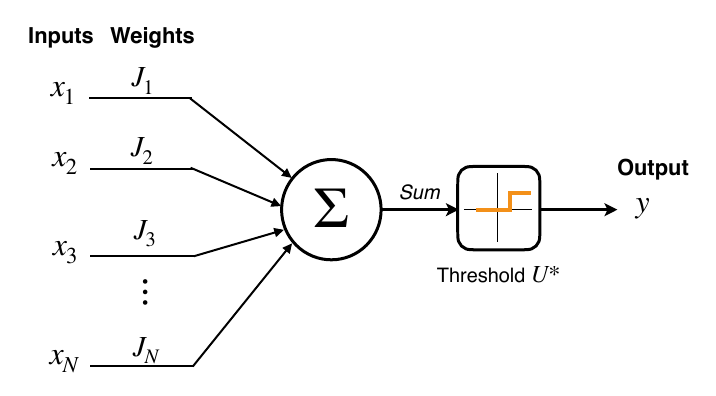
\includegraphics[width=0.8\linewidth]{img/McCulloch-Pitss_Neuron.png}
    \caption{Schematic representation of a MP neuron.}
    \label{fig:MPneuron}
\end{figure}


Before proceeding with the construction of networks of MP neurons it is worth noticing that there are two main classes of networks: \tbf{feed-forward networks} and \tbf{recurrent networks}. 
\\

\noindent
In the former, one distinguishes different layers of neurons, say layer 1, 2, ..., L and connections among them are directed in such a way that a neuron in layer n receives input from one (or more) neurons in layer n - 1 and contributes to the input to one (or more) neuron in layer n + 1. Thus, in this neural network, information only moves in one direction, forward, with respect to entry nodes, through nodes belonging to intermediate (if any) layers - these are also called hidden nodes - to exit nodes. Otherwise stated, in this case, $J_{ij} \neq 0$ and $J_{ji} = 0$ if neurons $j$ and $i$ belong, respectively, to layers $n - 1$ and $n$, but $J_{ki} \neq 0$ if neuron $k$ belongs to layer $n + 1$.
\\

\noindent
Conversely, in recurrent networks, connections are not directed and if a neuron $x_i$ is connected to a neuron $x_j$ then $x_i$ affects the state of $x_j$ which, in turn, affects the state of $x_i$ ; clearly, in this case, we have the existence of cycles. In this case it is convenient to label the MP neuron as well, namely to recast $y$ as $x_{N +1}$; accordingly, the vector $J$ is reshaped as a matrix $J = \{J_{ij} \}_{i,j=1,...,N +1}$, in such a way that eq. (\ref{eq:MPneuron}) turns into

\begin{equation}
    x_i = \theta(\sum\limits_{j=1}^{N +1} J_{ij} x_j - U_i^*) \quad i = 1, \ldots, N +1
\end{equation}

\noindent
where $J_{ij}$ therefore represents the amplification factor of the signal due to the $j$-th neuron on the $i$-th neuron and, in general, the effect can be asymmetric, namely $J_{ij} \neq J_{ji}$, and the sum possibly includes self-interactions, that is, $J_{ii}$ can be non zero. In the following we will only consider symmetric recurrent networks, where the connection matrix is symmetric, that is, $J_{ij} = J_{ji}$ for any $i, j$.

\subsection{Universality of McCulloch-Pitts neurons}

Here we will show that networks of MP neurons have universal computational capabilities in the sense that the operation of any finite, deterministic, digital-information processing machine can be emulated by a properly constructed network of MP neurons. Since the
basic logical units of digital machines can be constructed with MP neurons, all the theorems of computer science (on computability, Turing machines, etc.) that apply to such digital machines will also apply to MP neural networks.
\\

\noindent
We are going to demonstrate how any such machine can be reduced to a collection of simpler single-output binary machines:

\begin{itemize}
    \item Every finite digital machine can be regarded as a device that maps finite-dimensional binary input vectors $x \in \Omega \subseteq \{0, 1\}^N$ (representing characters, numbers, keys typed on a keyboard, camera images, etc.) onto finite dimensional binary output vectors $y \in \{0, 1\}^K$. Therefore every finite deterministic digital machine can be specified in full by specifying the output vector $y = S(x)$ for every possible input vector $x \in \Omega$, that is, by specifying the mapping $M:$
    $$ M : \Omega \rightarrow \{0, 1\}^K \quad M x = S(x) \quad \forall x \in \Omega $$
    \item Finally, we can always construct $K$ independent sub-machines $M_l \ ( l= 1, \ldots, K)$, each of which takes care of one of the $K$ output bits of the full mapping $M:$
    $$ M_l : \Omega \rightarrow \{0, 1\} \quad M_l x = S_l (x) \quad \forall x \in \Omega. $$
\end{itemize}


\noindent
We conclude that we are allowed to concentrate only on the question of whether it is possible to perform any single-output mapping $M : \Omega \subseteq \{0, 1\}^N \rightarrow \{0, 1\}$ with networks of MP neurons. This question will be answered in the affirmative in two steps: (i) we first show that any such single-output Boolean function of N variables can be expressed in terms of combinations of three logical operations performed on the inputs (AND, OR, NOT), (ii) the three elementary logical operations can be performed by MP neurons.
\\
For further details on these demonstrations, please refer to page 24 of the book.
\\

\noindent 
For statement (ii), the answer is positive only for $N=1$ that is, only for the trivial case of a single input variable $x \in \{0, 1\}$, we can check all possible operations $M : \{0, 1\} \rightarrow \{0, 1\}$ (of which there are four, to be denoted by $M_a , M_b, M_c,$ and $M_d$ ), and verify that one can always construct an equivalent MP neuron $y = S(x) = \theta(Jx - U^* )$, as outlined by Table \ref{tab:mappings}.

\begin{table}[h!]
    \centering
    \begin{tabular}{c|cccccccc}
    $x$ & $M_a(x)$ & $\theta(-1)$ & $M_b(x)$ & $\theta(-x + 1/2)$ & $M_c(x)$ & $\theta(x - 1/2)$ & $M_d(x)$ & $\theta(1)$ \\ \hline
    0 & 0 & 0 & 1 & 1 & 0 & 0 & 1 & 1 \\
    1 & 0 & 0 & 0 & 0 & 1 & 1 & 1 & 1 \\
    \end{tabular}
    \caption{The table shows the possible 4 mappings conceivable when $N = 1$.}
    \label{tab:mappings}
\end{table}

\noindent
For $N >1$, however, the answer is no. There are several ways for showing this. The simplest is to give first a counterexample for $N = 2$, which can subsequently be used to generate counterexamples for any $N \geq 2$, the so-called XOR operation (exclusive OR).

\begin{prop}
    No set of real numbers $\{J_1 , J_2, U^* \}$ exists such that
    $$ \theta(J_1 x_1 + J_2 x_2 - U^* ) = XOR(x_1 , x_2 ) \quad \forall (x_1 , x_2 ) \in \{0, 1\}^2 $$  
\end{prop}

\subsubsection{Geometric representation}

The set of all possible operations $ M : \{0, 1\}^N \rightarrow \{0, 1\} $ consists of all possible ways of assigning the output values 0 or 1 to the set of values $ \{0, 1\}^N $; since there are $ 2^N $ possible values in the domain of the function and each one can be assigned either 0 or 1, the total number of different operations is $ 2^{2^N} $.
\\

\noindent
A MP neuron, performing the operation
\begin{equation*}
    S : \{0, 1\}^N \rightarrow \{0, 1\} , \quad S(x) = \theta\left(\sum_{k=1}^{N} J_k x_k - U^* \right) \tag{3}
\end{equation*}
can be seen as dividing the space $ \mathbb{R}^N $ into two subsets which are separated by the hyperplane $ \sum\limits_{k=1}^{N} J_k x_k = U^* $. The information conveyed by the outcome of the operation of a MP neuron, given an input $ x \in \{0, 1\}^N $, is simply in which of the two subsets the corner $ x $ of the hypercube is located:

\begin{equation*}
    S(x)= \begin{cases}
        1 & \text{if } x \text{ is in the subset } \sum\limits_{k=1}^{N} J_k x_k > U^* \\
        0 & \text{if } x \text{ is in the subset } \sum\limits_{k=1}^{N} J_k x_k < U^*
    \end{cases} 
\end{equation*}

\noindent
For the moment, let us not worry about the pathological case where $x$ is on the separating plane.  For $N=2$, the hypercube is a square,. There are $2^2 = 4$ corners and $2^{2^2} = 16$ operations, $M : \{0, 1\}^2 \rightarrow \{0, 1\}$, that is, sixteen ways of colouring the four corners as we can see in Figure \ref{fig:operationsN2}.

\begin{figure}[H]
    \centering
    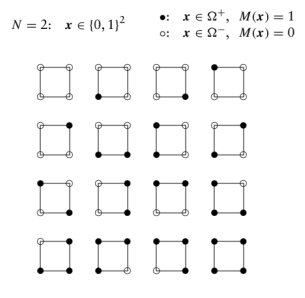
\includegraphics[width=0.5\linewidth]{img/operationsN2.png}
    \caption{All the possible operations for $N=2$.}
    \label{fig:operationsN2}
\end{figure}

\noindent
Next, by defining linear separability, we can see in Figure \ref{fig:linearlyseparable} which operations are linearly separable.

\begin{definicion}
    Let $X_1$ and $X_2$ be two sets of points in an n-dimensional Euclidean space.
    Then $X_1$ and $X_2$ are \tbf{linearly separable} if there exist $n + 1$ real numbers $w_1, w_2, \ldots, w_n , k$, such that every point $x \in X_1$ satisfies $\sum\limits_{i=1}^{n} w_i x_i > k$ and every point $x \in X_2$ satisfies $\sum\limits_{i=1}^{n} w_i x_i < k$. The expression $x \cdot w = k$ identifies a hyperplane that is referred to as the \tbf{separator hyperplane}.
    Setting $x_0 = 1$ and $w_0 = -k$, the separator hyperplane can be recast as $x\cdot w = 0$.
\end{definicion}

\begin{figure}[H]
    \centering
    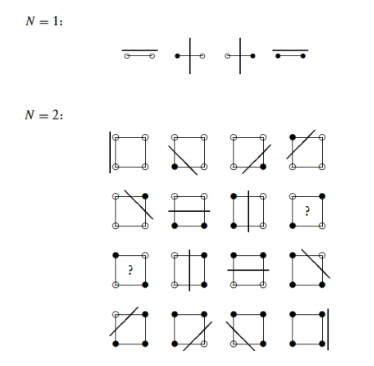
\includegraphics[width=0.5\linewidth]{img/linearlyseparable.png}
    \caption{Non linearly separable sets of points in a 2D space.}
    \label{fig:linearlyseparable}
\end{figure}

\section{Multilayer networks of MP neurons}
In accordance with what was previously agreed, a single MP neuron cannot realize every mapping $M : \{0, 1\}^N \longrightarrow \{0, 1\}$,
however, we also noticed that combinations of simple operations (each achievable by a
single MP neuron) can emulate any operation $M$, so in this section we are going to work with the ``grandmother-cell'' (or “Jennifer Aniston neuron”) concept. The main idea of this concept is that a single neuron, called the grandmother cell, is a hypothecal neuron that represents a complex but specific concept or object. It activates when a person "sees, hears, or otherwise sensibly discriminates" a specific entity.

\begin{notacion}
    The configuration of the middle (or `hidden') layer will be denoted as $y^{(1)} = (y_1^{(1)}, \ldots, y_L^{(1)})$; this notation allows a straightforward generalization in the case of multiple hidden layers, that is, $y^{(i)}=(y_1^{(i)}, \dots, y_j^{(i)}, \dots, y_n^{(i)})$ with $i\in \N$, whose sizes can, in principle, be arbitrary. \\
\end{notacion}

\noindent
Se busca una estructura de una MP neuron, es decir, se buscan weights $W_{ij}$ and firing thresholds $V_i$ for hidden neurons that satisfying
\begin{equation*}
    y_i^{(1)} (x) = \theta \left( \sum_{ j=1}^{N} W_{ij} x_j - V_i \right) = \delta_{x, x^i} \quad \text{with } x^i \in \Omega^+ \text{ and } x \in \{0, 1\}^N \\
\end{equation*}

\noindent
For the case $N=2$, let us see how to construct a function to differentiate the vectors that return $+1$ from those that return $-1$, so given $\Omega^+=\{x^1, x^2\}$ where $x^1=(1,0), x^2= (0,1)$ we can define

\begin{equation*}
    \sum_{j=1}^{2} (2x_j^i - 1)(2x_j - 1) =\sum_{j=1}^{2} 2(2x_j^i - 1)x_j - \sum_{j=1}^{2} (2x_j^i - 1) =
    \begin{cases}
        2 & \text{if } x = x^i \\
        \leq 0 & \text{otherwise}
    \end{cases}
\end{equation*}

\noindent
Here, the purpose is exploiting the knowledge of $\Omega^+$ and design the structure in such a way that, for each vector $x^i \in \Omega^+$, there is precisely one neuron $i$ in the middle (or `hidden') layer which produces an output $+1$, thereby signaling that the state of the output neuron is to be $+1$ when $x^i$ occurs as input, that is, $y_i^{(1)} = 1$ if $x = x^i$ where $x^i \in \Omega^+$ and $y_i^{(1)} = 0$ otherwise.
\\

\noindent
For the resolution of this case step by step, please refer to page 31 of the book, but we can see the main idea of the final sketch in Figure \ref{fig:multilayerN2}.

\begin{figure}[H]
    \centering
    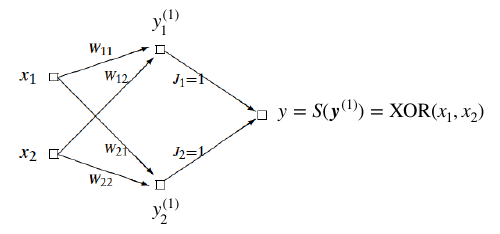
\includegraphics[width=0.6\linewidth]{img/multilayerN2.png}
    \caption{Schematic representation of a multilayer network of MP neurons.}
    \label{fig:multilayerN2}
\end{figure}

\subsection{General case}


We now give the general construction, which works for arbitrary input dimensions N
and for arbitrary operations $M: \{0,1\}^N\longrightarrow \{0,1\}$. Let $\Omega^+ = \{x \in \{0,1\}^N | M(x) = 1\}$ the set of all input vectors that are mapped to output value $+1 $ by the operation M, and $L := |\Omega^+|\in \N$. Then, we construt the neurons $y_i$ in the hidden layer such that the operation of each of them is defined as determining whether the input vector $x$ equals a neuron-specific prototype vector from $\Omega^+$, in other words, each $y_i^{(1)}$ is a \tbf{detector} for the prototype vector $x^i \in \Omega^+$, where its value would be $1$ if $x = x^i$ and $0$ otherwise.
\\

\noindent

\begin{definicion}
    For the construction of the associated grandmother neurons we need to define the \tbf{building block} $G$:

    \begin{equation*}
        G(x,x^*)=\theta \left( \sum_{i=1}^{N} (2x_i - 1)(2x_i^* - 1) - N + 1 \right) , \quad x, x^* \in \{0, 1\}^N
    \end{equation*} \\
\end{definicion} 

\noindent
Let's look at the main property that will interest us of this function.

\begin{prop}
    For the building block G defined above we have
    \begin{equation*}
        G(x, x^* )= 1 \iff x = x^*
    \end{equation*}
    Namely $G(x, x^* )= SAME(x,x^*)$.
    \begin{proof}
        If $x = x^*$, then
        \begin{equation*}
            G(x, x) = \theta \left( \sum_{i=1}^{N} (2x_i - 1)^2 - N + 1 \right) = \theta(1) = 1
        \end{equation*}
        Now we show that $G(x, x^* ) = 0$ as soon as $x \neq x^*$:
        \begin{equation*}
            \forall x_i, x_i^*\in \{0, 1\}: \quad (2x_i - 1)(2x_i^* - 1) = \begin{cases}
                1 & \text{if } x_i = x_i^* \\
                -1 & \text{if } x_i \neq x_i^*
            \end{cases}
        \end{equation*}
        Consequently,
        \begin{equation*}
            \sum_{i=1}^{N} (2x_i - 1)(2x_i^* - 1) = N - 2 \times (\text{number of indices } i \text{ with } x_i \neq x_i^* )
        \end{equation*}
        in such a way that
        \begin{equation*}
            x \neq x^* \implies \sum_{i=1}^{N} (2x_i - 1)(2x_i^* - 1) \leq N - 2 \implies G(x, x^* ) = 0
        \end{equation*}
        which completes the proof.
    \end{proof}
\end{prop}

\noindent
En este sentido, reestructurando el bloque $G$ se obtiene que la configuración buscada es
\begin{equation*}
    G(x, x^* ) = \theta \left( 2\sum_{i=1}^{N} (2x_i^* - 1)x_i - 2\sum_{i=1}^{N}x_i^* + 1 \right) 
\end{equation*}
thus, $G(x, x^*)$ is clearly of the MP form.

\noindent
We can now construct our two-layer network from these building blocks, by assigning to each vector $x \in \Omega^+$ a hidden neuron of the form $G(x, x^*)$
\begin{equation*}
    \Omega^+ = \{x \in \{0, 1\}^N |M (x) = 1\} = \{x^1 , x^2, \ldots, x^{L-1} , x^L\}
\end{equation*}
\begin{equation*}
    \forall i \in \{1, \ldots, L\} \quad y_i^{(1)} : \{0, 1\}^N \rightarrow \{0, 1\} \quad y_i^{(1)} = G(x, x^i ).
\end{equation*}
The required operation of the output neuron S, finally, is to simply detect whether or not any
of the hidden layer neuron states $y_i^{(1)}$ equals one. Our final result is the following network
\begin{equation*}
    y_i^{(1)} (x) = \theta \left( \sum_{ j=1}^{N} W_{ij} x_j - V_i \right), \quad y = S(y^{(1)})=\theta \left( \sum_{i=1}^{L} y_i^{(1)} - \frac{1}{2} \right)
\end{equation*}
where $W_{ij} = 2(2x_j^i - 1)$ and $V_i = 2 \sum\limits_{j=1}^{N} x_j^i - 1$. Destacar que tenemos $U^*= \frac{1}{2}$ y $J_i=1, \forall i=1, \dots, L$ en la neurona de salida.
    
\section{The perceptron}

\noindent
For a MP neuron $S(x) = \theta(J \cdot x - U^*)$ learning means the adaptation of the set of connections $\{J_i\}_{i=1}^{N}$ and the threshold $U^*$, in order to improve the accuracy in the execution of a given task $M : \{0,1\}^N \rightarrow \{0,1\}$.
\\


\noindent
We don't know the task $M$ explicitly, we only have some available examples provided by some ``teacher'' of ``questions'' (input vectors $x \in \{0,1\}^N$) with corresponding ``answers'' (the associated output values $M(x)$), and the main idea is that $S(x)$ classifies examples $x\in\{0,1\}^N$ ``mimicking'' $M(x)$. A so-called ``online'' training session consists of iterating the following procedure:

\begin{itemize}
    \item STEP 1: Draw at random a question $x \in \Omega$
    \item STEP 2: Check whether teacher and student agree on the answer:
    \begin{itemize}
        \item if $M (x) = S(x)$: do nothing, return to STEP 1.
        \item if $M (x) \neq S(x)$: modify parameters
        \begin{equation*}
            \begin{array}{ccc}
                J & \longmapsto & J + \Delta J(J, U^* ; x, M(x)) \\
                U & \longmapsto & U^* + \Delta U^*(J, U^* ; x, M(x))
            \end{array}
        \end{equation*}
        then return to STEP 1.
    \end{itemize}
\end{itemize}

\begin{definicion}(Experience)
    Llamaremos \tbf{experience} al conjunto de ejemplos $\{x^{(i)}, M(x^{(i)})\}_{i=1,\dots,P}$ que el perceptrón utiliza para aprender a aproximar la función objetivo $M : \{0, 1\}^N \rightarrow \{0, 1\}$.
\end{definicion}

\begin{definicion}(Performance)
    We define the \tbf{performance} of the perceptron on a given experience as la exactitud de la función $S$ respecto a la función objetivo $M$ en los $P$ ejemplos que componen la experiencia:
    \begin{equation*}
        dist(\{x^{(i)}, M(x^{(i)})\}_{i=1,\dots,P})
    \end{equation*}
\end{definicion}

\noindent
The problem one faces is how to choose an appropriate recipe $(\Delta J , \Delta U^* )$ for updating the neuron’s parameters that will achieve this. A perceptron is defined as a MP neuron which learns according to the following rule (perceptron learning rules) for updating its parameters:
\begin{equation*}
    \begin{cases}
        S(x) = 1 , M (x) = 0 \Rightarrow \Delta U^* = 1 , \Delta J = -x \\
        S(x) = 0 , M (x) = 1 \Rightarrow \Delta U^* = -1 , \Delta J = x
    \end{cases}
\end{equation*}

\begin{teo}(Perceptron convergence theorem, Rosenblatt [1958])
    If the task M is linearly separable, then the above procedure will converge in a finite number of modification steps to a stationary configuration, where $\forall x \in \Omega : S(x) = M (x)$.
\end{teo}

\section{Recurrent networks of MP neurons}

\noindent
First, having in mind a network of MP neurons that mutually interact each other, we can look at (\ref{eq:MPneuron}) as an evolutionary rule which can be applied in turn to all the neurons making up the network and which can be possibly iterated. We therefore introduce a dependence on a time variable as follows
\begin{equation} \label{eq:recurrentMP}
    x_i (t + \Delta t) = \theta\left( \sum_{j=1}^{N} J_{ij} x_j (t) - U_i^* \right)
\end{equation}
where $\Delta t$ represents the refractory time.

\begin{notacion} 
    From now on, we will use the following notation $U_i(t)= \sum\limits_{j=1}^{N} J_{ij} x_j (t)$ to indicate the post-synaptic potential acting on neuron $i$ at time $t$. \\
\end{notacion}

\noindent
En el modelo anterior de McCulloch-Pitts (MP), la neurona es un robot predecible. Compara su entrada $U_i(t)$ con un umbral fijo $U_i^*$. Si $U_i(t) > U_i^*$, se activa; si no, no. El problema es que este sistema se queda atascado en mínimos locales (memorias espurias). La solución estocástica es introducir "ruido" para permitir que la neurona "se equivoque" a propósito, dándole la capacidad de saltar fuera de esos valles de energía. \\

\noindent 
Aplicamos ahora la teoría de Procesos Estocásticos introduciendo $z_i(t)$ que es una variable aleatoria que actúa como fuente de ``ruido térmico'' que recibe la neurona $i$ en el instante $t$. \\

\subsection{Stochastic neurons}

\begin{definicion}(Sthocastic neurons)
    Dada la definición de la neurona MP recurrente en (\ref{eq:recurrentMP}), una \tbf{neurona estocástica} es aquella que tiene un umbral fluctuante dado de la siguiente manera
    \begin{equation*}
        U_i^* (t) = U_i^* -\dfrac{1}{2} Tz_i (t)
    \end{equation*}
    donde $T\in\R^+$ es la \tbf{controlador de la magnitud del ruido} (o también llamado \tbf{temperatura}) y $z_i(t)$ es una \tbf{variable aleatoria} independiente e idénticamente distribuida (i.i.d.), es decir, $z_i (t) \sim_{idd} P, \ \forall i=1, \dots, N$. Tomaremos estas propiedades como supuestos básicos en el modelo:
    \begin{multicols}{2}
        \begin{itemize}
            \item $\E[z_i(t)] = \overline{z_i(t)} = 0$
            \item $\E[z_i(t)^2] = \overline{z_i(t)^2} = 1$
        \end{itemize}
    \end{multicols}
\end{definicion}

\noindent
Cabe destacar que la esperanza de la diferencia del umbral fluctuante al cuadrado es
\begin{equation*}
    \E[(U_i^* (t) - U_i^*)^2] = \E\left[\left(-\dfrac{1}{2} Tz_i (t)\right)^2\right] = \dfrac{T^2}{4} \E[z_i(t)^2] = \dfrac{T^2}{4}
\end{equation*}
por lo que el parámetro $T$ controla la magnitud de las fluctuaciones del umbral, es decir, la aleatoriedad de la neurona estocástica es controlada por $T$.

\noindent
A partir de ahora el estado de la neurona estocástica $i$ en el instante $t + \Delta t$ viene dado por
\begin{equation*}
    x_i (t + \Delta t) = \theta\left( U_i(t)-U_i^*(t)\right)
\end{equation*}

\subsection{Stochastic symmetric neurons}
El objetivo será mapear nuestro sistema de neuronas estocásticas con activación $\{0,1\}$ a un sistema de neuronas simétricas con activación $\{-1, +1\}$, ya que este último es más sencillo de analizar. Para ello, teniendo en cuenta el \tbf{modelo de neuronas de Ising} sabemos que la neurona $\sigma_i$ se activa (pasa a $+1$) si la entrada neta que recibe es positiva, es decir, 
\begin{equation*}
    \sum\limits_{k=1}^{N} J_{ik} \sigma_k  +h_i>0 \Longleftrightarrow \sum\limits_{k=1}^{N} J_{ik} \sigma_k > -h_i
\end{equation*}
donde $h_i$ es su preferencia personal o un estímulo que viene de fuera de la red. Por tanto, tomando la conversión de las neuronas $x_i(t) = \dfrac{1}{2}[\sigma_i(t)+1]$ (para pasar de sistema $\{0,1\}$ a $\{-1,+1\}$) tenemos que
\begin{equation*}
    \sum\limits_{k=1}^{N} J_{ik} x_k > U_i^* \iff \sum\limits_{k=1}^{N} J_{ik} \dfrac{1}{2}[\sigma_i(t)+1] > U^* \Longleftrightarrow \sum\limits_{k=1}^{N} J_{ik} \sigma_k > 2U_i^* - \sum\limits_{k=1}^{N} J_{ik}
\end{equation*}

\noindent
Igualando las dos expresiones obtenidas, tenemos que el mapeo al nuevo sistema simétrico es 
\begin{equation}\label{eq:mapeoIsingModel}
    \left\{
    \begin{array}{l}
        x_i(t) = \dfrac{1}{2}[\sigma_i(t)+1] \\
        U_i^* = \dfrac{1}{2}\left( \sum\limits_{k=1}^{N} J_{ik} - h_i \right)
    \end{array}\right.
\end{equation}


\noindent
The stochastic version of the MP model is the following
\begin{equation*}
    x_i (t + \Delta t) = \theta\left( \sum_{j=1}^{N} J_{ij} x_j (t) - U_i^* + \dfrac{1}{2} T z_i (t) \right)
\end{equation*}
thereby becomes
\begin{align*}
    \dfrac{1}{2}[\sigma_i (t + \Delta t) + 1] = \theta\left( \sum_{k=1}^{N} J_{ik} \dfrac{1}{2}[\sigma_k (t) + 1] - \dfrac{1}{2}\left( \sum_{k=1}^{N} J_{ik} - h_i \right) + \dfrac{1}{2} T z_i (t) \right) \Longrightarrow \\
    \Longrightarrow \dfrac{1}{2}[\sigma_i (t + \Delta t) + 1] = \theta\left( \dfrac{1}{2} \sum_{k=1}^{N} J_{ik} \sigma_k (t) + \dfrac{1}{2}h_i + \dfrac{1}{2}T z_i (t) \right)
\end{align*}
then
\begin{equation*}
    \sigma_i (t + \Delta t) = sgn\left( \varphi_i (t) + T z_i (t) \right) \quad \text{where} \quad \varphi_i (t) = \sum_{k=1}^{N} J_{ik} \sigma_k (t) + h_i
\end{equation*}

\begin{definicion}(Stochastic version of the MP model)
    The \tbf{stochastic version of the MP model} for a network of $N$ symmetric neurons is defined by the following evolutionary rule:
    \begin{equation*}
        \sigma_i (t + \Delta t) = sgn\left( \varphi_i (t) + T z_i (t) \right) \quad \text{where} \quad \varphi_i (t) = \sum_{k=1}^{N} J_{ik} \sigma_k (t) + h_i
    \end{equation*}

    \noindent
    so $sgn(x > 0) = +1$, $sgn(x < 0) = -1$; $sgn(0)$ is drawn randomly from $\{-1, +1\}$. The quantity $\varphi_i (t)$ is called the \tbf{local field}. The first term of $\varphi_i (t)$ is called the \tbf{internal field} and is due to the first neighboring neurons, that is to other elements of the system; the second term is referred to as \tbf{external field} because it acts as a bias, independent of the neuronal configuration and favouring either one of the possible states. \\
\end{definicion}

\noindent
Lo que hemos hecho aqui realmente es unir el concepto de MP neurona estocástica con el modelo de Ising, obteniendo así una neurona estocástica simétrica. A partir de aquí podemos analizar la probabilidad de que la neurona $i$ tome el valor $\sigma_i (t + \Delta t) = \pm 1$.\\

\noindent
La probabilidad de que la neurona $i$ tome el valor $\sigma_i (t + \Delta t) = +1$ se puede expresar en términos de la distribución $\mathcal{P}(z)$ de la variable aleatoria $z_i(t)$. Para las distribuciones simétricas del ruido, es decir, $\mathcal{P}(z)=\mathcal{P}(-z) \ \forall z$ tenemos
\begin{align*}
    P[\sigma_i (t + \Delta t) = 1] &= P[\varphi_i(t + \Delta t) + T z_i(t) > 0] = \int_{-\varphi_i (t)/T}^{\infty} \mathcal{P}(z) \, dz \\
    P[\sigma_i (t + \Delta t) = -1] &= \int_{-\infty}^{-\varphi_i (t)/T} \mathcal{P}(z) \, dz = \int_{\varphi_i (t)/T}^{\infty} \mathcal{P}(z) \, dz,
\end{align*}
\noindent
We can now combine the two probabilities into the single expression:
\begin{equation*}
    P[\sigma_i(t + \Delta t) = \pm 1] = g(\pm \varphi_i (t)/T )
\end{equation*}
with
\begin{equation*}
    g(x) = \int_{-\infty}^{x} \mathcal{P}(z) dz = \dfrac{1}{2}+ \int_{0}^{x} \mathcal{P}(z) dz.
\end{equation*}

\noindent
The function $g(x)$ is a cumulative distribution function and it has the following properties:
\begin{itemize}
    \item[(i)] $g(x) + g(-x) = 1$
    \item[(ii)] $\lim\limits_{x\to-\infty} g(x) = 0, \ g(0) = 1/2, \ \  \lim\limits_{x\to\infty} g(x) = 1$
    \item[(iii)] $g' (x) = P(x) : \ g' (x) \geq 0 \ \forall x, \ g' (-x) = g'(x) \ \forall x, \ \lim\limits_{x\to\pm\infty} g' (x) = 0.$
\end{itemize}

\noindent 
Una elección usual de la distribución del ruido es la distribución normal estándar, es decir, \mbox{$z\sim \mathcal{N}(0,1)$} con función de densidad de probabilidad
\begin{equation*}
    \mathcal{P}(z) = \dfrac{1}{\sqrt{2\pi\sigma}} e^{-\dfrac{(z-\mu)^2}{2\sigma^2}}
\end{equation*}
donde $\mu = 0$ y $\sigma = 1$, por supuesto al inicio de esta sección y por tanto tenemos

\begin{equation*}
    g(x) = \dfrac{1}{2} +  \int_{0}^{x}\dfrac{1}{\sqrt{2\pi}} e^{-\dfrac{z^2}{2}} dz = \dfrac{1}{2} \left[ 1 + erf\left( \dfrac{x}{\sqrt{2}} \right) \right]
\end{equation*}


\begin{definicion}
    La función $erf(z)$ se define como el área bajo una curva Gaussiana específica (normalizada de una manera particular), desde 0 hasta un valor $z$:
    \begin{equation*}
        erf(z) = \dfrac{2}{\sqrt{\pi}} \int_{0}^{z} e^{-t^2} dt
    \end{equation*}
    Mide que tan probable es que una variable Gaussiana con media $\mu = 0$ y varianza $\sigma^2 = \frac{1}{2}$, caiga entre $-z$ y $+z$.
\end{definicion}





